\documentclass[conference]{IEEEtran}
\IEEEoverridecommandlockouts
\usepackage{cite}
\usepackage{amsmath,amssymb,amsfonts}
\usepackage{algorithmic}
\usepackage{graphicx}
\usepackage{textcomp}
\usepackage{xcolor}
\usepackage{booktabs}
\usepackage{hyperref}
\usepackage{caption}

\begin{document}

\title{Auditory Hallucinations and Causal Uncertainty: \\ An Information-Theoretic Approach to Computational Psychiatry}

\author{\IEEEauthorblockN{Erick Oduniyi}
\IEEEauthorblockA{\textit{Chaos Hearing Project} \\
\textit{MIT Media Lab}\\
Cambridge, MA \\
eoduniyi@mit.edu}
}

\maketitle

\begin{abstract}
Computational psychiatry frames perceptual anomalies, such as hallucinations and sensory overload, as imbalances in predictive coding and Bayesian inference. This paper bridges the gap between acoustic information theory and psychiatric modeling by exploring how the manipulation of a sound's causal uncertainty ($H_{cu}$) interacts with internal generative priors. By algorithmically optimizing a sound to maximize the entropy of its causal likelihood, we can simulate the environmental conditions that trigger maladaptive perception. Under the Free Energy Principle, a neurotypical brain remains uncertain when presented with high-entropy audio; however, an architecture modeled on schizophrenia, characterized by overly precise priors, will forcefully resolve this uncertainty by hallucinating a spurious cause. Conversely, architectures modeling autism display over-precise weighting of the ambiguous sensory evidence, failing to contextualize it. This synthesis provides a mathematical and cyber-physical framework for understanding how structural sound parameters interact with cognitive processing in both healthy and disordered states.
\end{abstract}

\begin{IEEEkeywords}
computational psychiatry, causal uncertainty, information theory, predictive coding, auditory hallucinations, free energy principle
\end{IEEEkeywords}

\section{Introduction}

The subjective experience of hearing is not a passive reception of acoustic waveforms, but an active, generative process of causal inference. When we hear a sound, our auditory cortex attempts to infer its source---a process known in ecological psychology as estimating causal uncertainty~\cite{b1}. Recent work by Boger et al. (2021) demonstrated that this intrinsic causal uncertainty can be systematically manipulated by optimizing a sound's acoustic parameters (such as pitch, playback speed, and reverberation) to flatten the classification confidence of an audio neural network~\cite{b1}.

Simultaneously, the field of computational psychiatry has coalesced around the Free Energy Principle and predictive coding as unified frameworks for understanding mental illness~\cite{b2}. In this paradigm, perception is the optimal precision-weighted combination of sensory evidence (the likelihood) and internal expectations (the prior). Hallucinations and sensory processing disorders arise when this precision-weighting mechanism becomes imbalanced.

This paper bridges these two domains. We argue that Boger et al.'s optimization of causal uncertainty is mathematically equivalent to maximizing the Shannon entropy of the sensory likelihood function. By feeding this mathematically ambiguous audio into Bayesian models of varying psychiatric conditions, we can simulate how different cognitive architectures attempt to resolve the ambiguity, leading directly to the phenomenon of auditory hallucinations.

\section{Information Theory and Causal Uncertainty}

We define causal uncertainty, $H_{cu}$, as the Shannon entropy of the posterior distribution over possible causes $C$ given a sound sequence $S$:
\begin{equation}
    H(C|S) = -\sum_{c \in C} P(c|s) \log_2 P(c|s)
\end{equation}

In a clear, unambiguous sound environment, the distribution $P(c|s)$ is sharply peaked around the true cause (e.g., a dog barking), resulting in low entropy. The optimization procedure introduced in~\cite{b1} acts as an adversarial attack on this certainty. By iteratively perturbing the sound's low-level acoustic features and penalizing label distance, the optimization process deliberately flattens the likelihood function, driving the entropy toward a theoretical maximum where multiple causes are equally probable.

\begin{figure}[htbp]
\centering
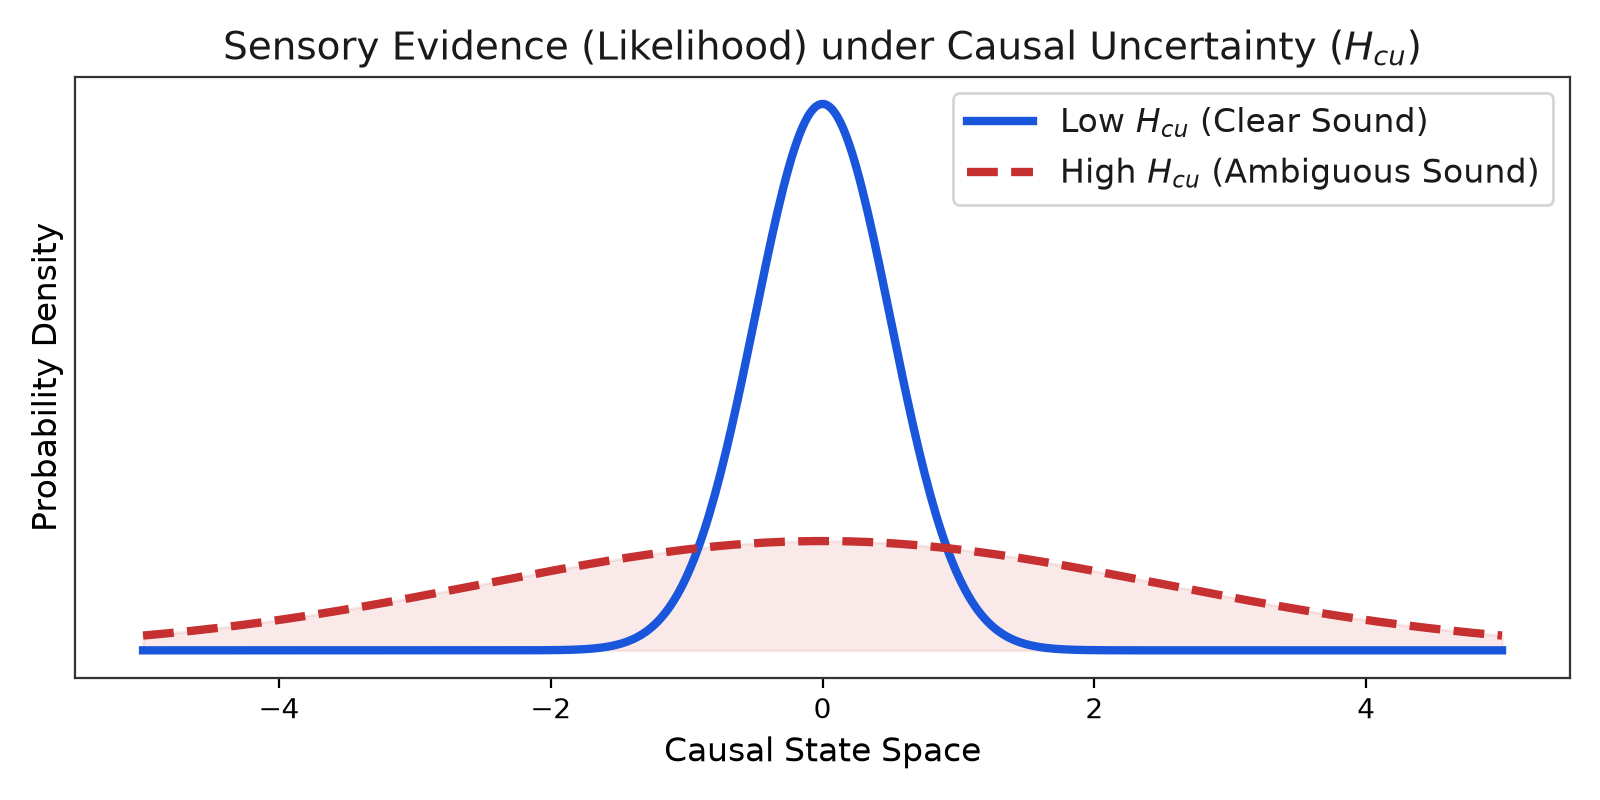
\includegraphics[width=0.95\columnwidth]{figures/causal_uncertainty_likelihood.png}
\caption{The effect of manipulating causal uncertainty ($H_{cu}$). The blue curve represents clear sensory evidence (low entropy likelihood). The red dashed curve represents the manipulated sound where acoustic optimization has deliberately flattened the likelihood function, making the source ambiguous.}
\label{fig:hcu}
\end{figure}

\section{Predictive Coding and Precision Weighting}

In the predictive coding framework, the brain minimizes surprise (free energy) by updating its internal models to match the sensorium. Assuming Gaussian distributions for simplicity, the posterior percept ($\mu_{post}$) is a precision-weighted sum of the sensory likelihood ($\mu_{lik}$) and the internal prior ($\mu_{prior}$):
\begin{equation}
    \mu_{post} = \frac{\pi_{lik}\mu_{lik} + \pi_{prior}\mu_{prior}}{\pi_{lik} + \pi_{prior}}
\end{equation}
where precision $\pi$ is the inverse variance ($1/\sigma^2$).

When $H_{cu}$ is artificially raised (i.e., $\pi_{lik}$ approaches 0), the posterior becomes heavily dependent on the precision of the prior, $\pi_{prior}$. This dynamic is the crux of computational psychiatry~\cite{b2}.

\section{Psychiatric Models of Ambiguity Resolution}

We can simulate the perceptual outcomes of presenting a high-$H_{cu}$ sound to different cognitive architectures by manipulating their respective precision weightings.

\begin{figure*}[tbp]
\centering
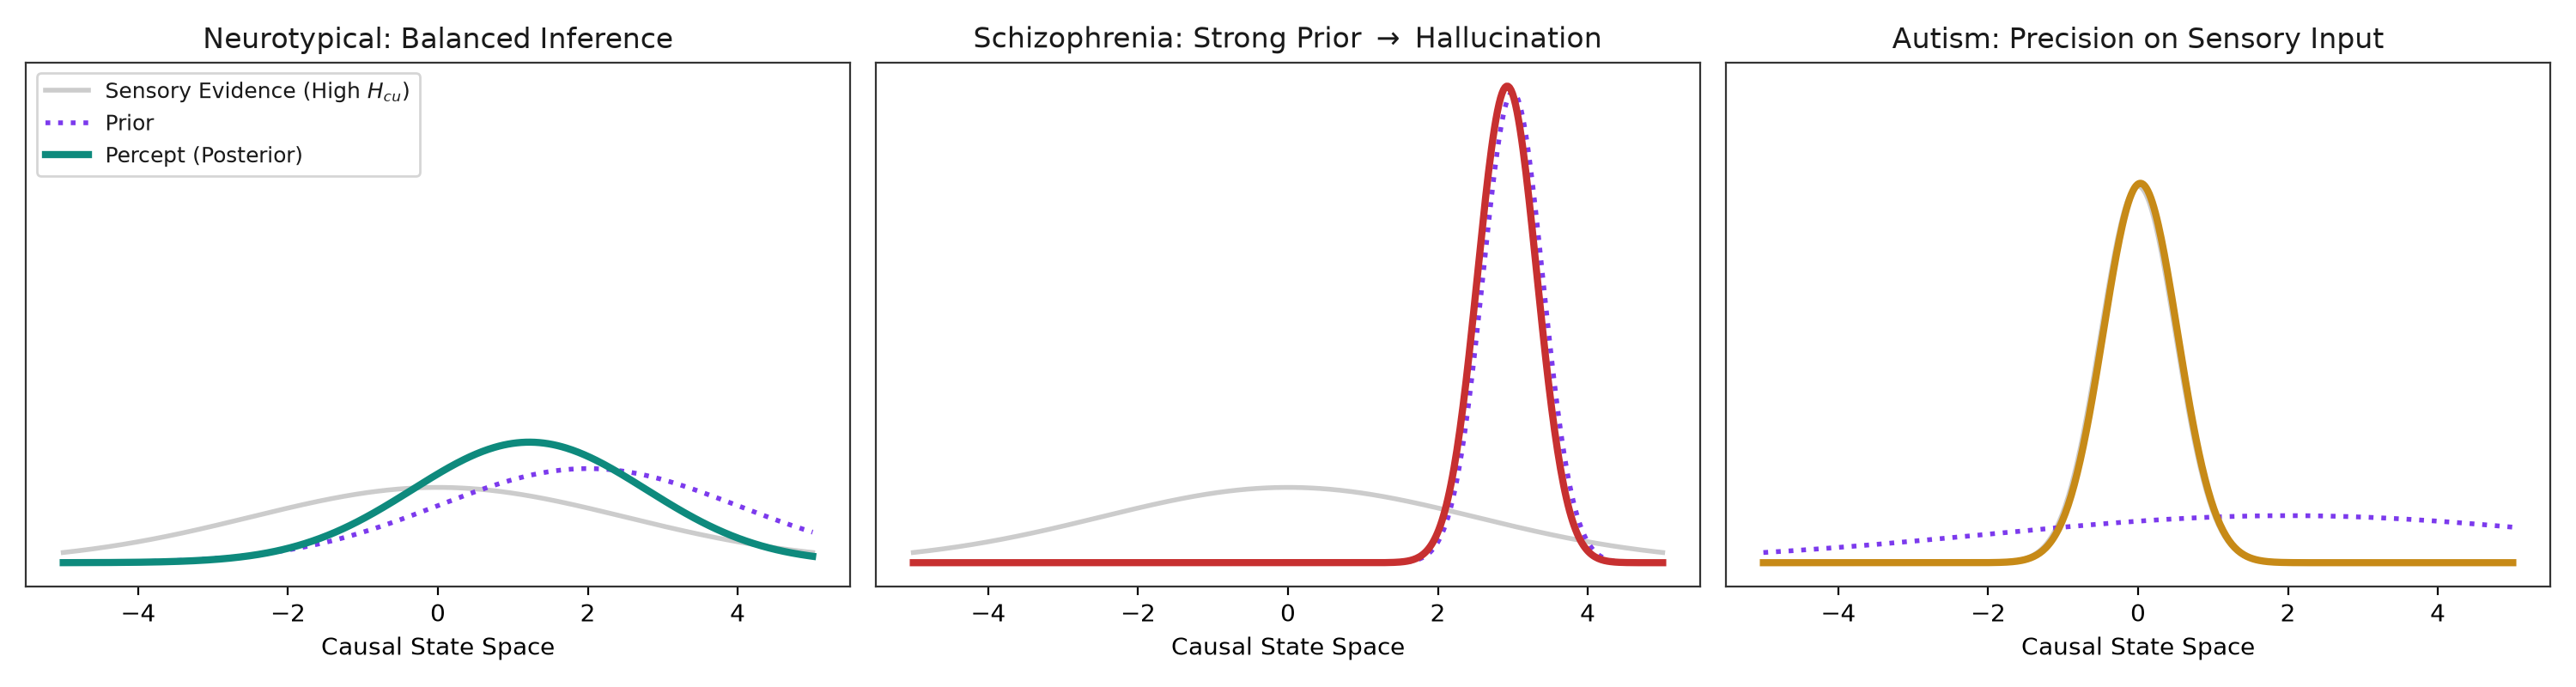
\includegraphics[width=0.95\textwidth]{figures/predictive_coding_psychiatry.png}
\caption{Simulated Bayesian inference across three cognitive architectures when presented with high causal uncertainty ($H_{cu}$) audio. (Left) A neurotypical system balances a weak prior against the broad likelihood, resulting in an uncertain percept. (Middle) A schizophrenia model relies on an overly precise (maladaptive) prior, ignoring the ambiguity of the sensory input and confidently hallucinating a specific cause. (Right) An autism model assigns inappropriately high precision to the sensory input, failing to integrate prior context and resulting in sensory overload.}
\label{fig:psychiatry}
\end{figure*}

\subsection{The Neurotypical Baseline}
In a healthy cognitive architecture, the prior is moderately precise, reflecting general statistical expectations about the acoustic environment. When presented with high-$H_{cu}$ sensory evidence (a broad likelihood), the resulting posterior is also broad (Figure~\ref{fig:psychiatry}, left). The individual accurately perceives that they do not know what caused the sound. The ambiguity is maintained without distress.

\subsection{Schizophrenia and Auditory Hallucinations}
Computational models of schizophrenia, particularly those focusing on hallucinations and delusions, posit an imbalance where internal generative priors become overly precise ($\pi_{prior} \gg \pi_{lik}$)~\cite{b3}. When this architecture encounters the optimized, high-$H_{cu}$ sound, the broad sensory likelihood offers no resistance to the overwhelming force of the prior. 

\subsection{Autism and Sensory Overload}
Conversely, some predictive coding models of autism spectrum disorder (ASD) suggest a failure to attenuate sensory precision, leading to a state where sensory evidence is consistently over-weighted ($\pi_{lik} \gg \pi_{prior}$)~\cite{b4}. 

When presented with ambiguous audio, this architecture treats the high-entropy input as if it were highly informative and precise (Figure~\ref{fig:psychiatry}, right). The failure to use the prior to smooth over or contextualize the noise results in an inability to filter out irrelevant acoustic details, directly modeling the phenomenon of auditory sensory overload.

\subsection{Alarm Fatigue and the ``Cry Wolf'' Effect}
Beyond inherent neurodevelopmental or psychiatric conditions, precision weighting is dynamically modulated by environmental statistical history. In safety-critical human-machine interfaces, operators exposed to high rates of non-actionable alerts experience \emph{alarm fatigue} (the ``cry wolf'' effect). 

Mathematically, non-critical stochastic noise deforms the state probability density function, creating phenomenological boundary crossings or P-bifurcations. When an operator repeatedly encounters these false positives, the predictive coding architecture adapts by exponentially decaying the sensory precision weight ($\pi_{lik} \to 0$). When a true catastrophic failure occurs (a dynamical D-bifurcation), the posterior belief of danger fails to breach the action threshold because the prior belief of a false alarm dominates the inference. Alarm fatigue is thus formalised as an acquired, localized sensory desensitization induced by noise-driven P-bifurcations.

\section{Conclusion}

The optimization of causal uncertainty in sound objects is more than an interface design tool; it provides a rigorous mathematical environment for testing theories of computational psychiatry. By defining $H_{cu}$ as Shannon entropy and feeding these manipulated signals into Bayesian predictive coding frameworks, we demonstrate how structural properties of sound interact with cognitive vulnerabilities. This intersection of acoustic information theory and psychiatry offers profound insights into how the brain constructs its reality, and why that construction sometimes fails.

\begin{thebibliography}{00}
\bibitem{b1} T. Boger, I. Ananthabhotla, and J. A. Paradiso, ``Manipulating Causal Uncertainty in Sound Objects,'' in \emph{Audio Mostly 2021}, Sep. 2021, pp. 9--15.
\bibitem{b2} K. Friston, ``The free-energy principle: a unified brain theory?'' \emph{Nature Reviews Neuroscience}, vol. 11, no. 2, pp. 127--138, 2010.
\bibitem{b3} P. C. Fletcher and C. D. Frith, ``Perceiving is believing: a Bayesian approach to explaining the positive symptoms of schizophrenia,'' \emph{Nature Reviews Neuroscience}, vol. 10, no. 1, pp. 48--58, 2009.
\bibitem{b4} E. Pellicano and D. Burr, ``When the world becomes `too real': a Bayesian explanation of autistic perception,'' \emph{Trends in Cognitive Sciences}, vol. 16, no. 10, pp. 504--510, 2012.
\end{thebibliography}

\end{document}
